% !TEX TS-program = lualatex
% !TEX encoding = UTF-8 Unicode

% This is a simple template for a LaTeX document using the "article" class.
% See "book", "report", "letter" for other types of document.

\documentclass[10pt, twocolumn]{article} % use larger type; default would be 10pt

\usepackage[utf8]{inputenc} % set input encoding (not needed with XeLaTeX)
\usepackage{fontspec}
\setmainfont{Georgia}
\setsansfont{Georgia}
\setmonofont{Georgia}
%\usepackage[none]{hyphenat}
\usepackage{hyphenat}

%%% Examples of Article customizations
% These packages are optional, depending whether you want the features they provide.
% See the LaTeX Companion or other references for full information.

%%% PAGE DIMENSIONS
\usepackage{geometry} % to change the page dimensions
\geometry{a4paper, left=17.5mm, right=17.5mm, textwidth=85mm,columnsep=5mm, top=17.5mm}
\setlength{\parindent}{0pt}
% or letterpaper (US) or a5paper or....
% \geometry{margin=2in} % for example, change the margins to 2 inches all round
% \geometry{landscape} % set up the page for landscape
%   read geometry.pdf for detailed page layout information

\usepackage{subcaption}
\usepackage{graphicx} % support the \includegraphics command and options

\usepackage[parfill]{parskip} % Activate to begin paragraphs with an empty line rather than an indent

%%% PACKAGES
\usepackage{booktabs} % for much better looking tables
\usepackage{array} % for better arrays (eg matrices) in maths
\usepackage{paralist} % very flexible & customisable lists (eg. enumerate/itemize, etc.)
\usepackage{verbatim} % adds environment for commenting out blocks of text & for better verbatim
%\usepackage{subfig} % make it possible to include more than one captioned figure/table in a single float
\usepackage{amsmath}
% These packages are all incorporated in the memoir class to one degree or another...
\usepackage{lipsum}
%\usepackage{caption}
\usepackage{listings}

%%% HEADERS & FOOTERS
\usepackage{fancyhdr} % This should be set AFTER setting up the page geometry
\pagestyle{fancy} % options: empty , plain , fancy
\renewcommand{\headrulewidth}{0pt} % customise the layout...
\lhead{}\chead{}\rhead{}
\lfoot{}\cfoot{\thepage}\rfoot{}

%%% SECTION TITLE APPEARANCE
%\usepackage{sectsty}
%\allsectionsfont{\sffamily\mdseries\upshape} % (See the fntguide.pdf for font help)
% (This matches ConTeXt defaults)

%%% ToC (table of contents) APPEARANCE
\usepackage[nottoc,notlof,notlot]{tocbibind} % Put the bibliography in the ToC
\usepackage[titles,subfigure]{tocloft} % Alter the style of the Table of Contents
\renewcommand{\cftsecfont}{\rmfamily\mdseries\upshape}
\renewcommand{\cftsecpagefont}{\rmfamily\mdseries\upshape} % No bold!
\usepackage{authblk}

\usepackage{float}

\newcommand{\overbar}[1]{\mkern 1.5mu\overline{\mkern-1.5mu#1\mkern-1.5mu}\mkern 1.5mu}

%%% END Article customizations

%%% The "real" document content comes below...

\title{\textbf{Investigation of fractal dimension in modified diffusion-limited aggregation algorithms}}
\author{Candidate Number: 24669}
\affil{Department of Physics, University of Bath, Bath BA2 7AY, United Kingdom}
%\date{} % Activate to display a given date or no date (if empty),
         % otherwise the current date is printed 

\begin{document}
\twocolumn[
 \begin{@twocolumnfalse}
\maketitle
\begin{abstract}
  Diffusion-limited aggregation (DLA) clusters also known as Brownian trees are branching fractal objects that arise from the aggregation of random-walking particles. A fractal is an object with non-integer dimension, its uniform mass density grows by a non-integer power of its linear size. Because of their self-similar properties and scale invariance DLA systems are used to model a variety of physical and biological processes. As such, the effects of the conditions in a DLA simulation on the resulting DLA cluster are well studied. This report examines the fractal dimension of DLA clusters generated from an initial 'seed' particle with varying probability of particle adherence. We compare the efficacy of two methods of deriving fractal dimension $d_f$ from the particle number $N_c$ and linear size $r_{max}$ of simulated clusters - determining the mean fractal dimension $\overbar{d_f}$ of a sample of DLA clusters to be 1.733 $\pm$ 0.004. Further, we find a negative correlation between the probability of particle adhesion and fractal dimension in concurrence with other literature.

\bigskip
\end{abstract}
\end{@twocolumnfalse}
]
\medskip

\section*{Introduction}
  The primary mechanism in diffusion-limited aggregation (DLA) systems is Brownian motion - named for early contributor Robert Brown \cite{Pearle_2010} and later studied by Einstein \cite{Einstein_1905}, whereby fluctuations within a medium impart forces on diffuse particles, resulting in seemingly random motion. \textit{Ab-initio} simulation of all of the constituent particles of a diffuse substance in a medium is computationally expensive, however it has been shown by Donsker's theorem that Brownian motion is well approximated by the stochastic Weiner process. The Weiner process can be modelled as a discrete random walk on a lattice in the limit as the lattice constant tends to zero (the scaling limit). Thus, for practical computation a discrete random walk is a sufficient approximation of Brownian motion. Additionally some physical systems have characteristic length scales (e.g. electrodeposition \cite{Shaikh_2022}), further justifying their approximation by a discrete random walk.

  DLA models produce DLA clusters, also known as Brownian trees, fractal objects that grow by adhering random-walking particles to one another. A common initial condition in the study of natural systems is a single initial particle onto which the diffuse particles attach after random walking towards the structure from some starting radius. The single particle initial state model was first proposed by Eden in 1961 \cite{Eden_1961} to describe the growth of bacterial colonies from as a stochastic process. Further developments by Witten and Sander in 1981 \cite{Witten_1981} on metal-particle aggregation introduced clustering by Brownian motion to the Eden model, often referred to as 'classical' DLA. They also show DLA clusters to be critical phenomena arising from irreversible growth processes rather than an equilibrium ensemble. Other studies have extended the model to additional spatial dimensions \cite{Ball_1984}, or varying geometries such as curved \cite{Choi_2011} and spherical \cite{Tenti_2021} surfaces. Furthermore, Laplacian growth theory has succeeded in describing varying DLA systems along with other fractal generating systems under a single universality class \cite{Mathiesen_2005, Carlock_2016}.

  DLA systems and the corresponding fractal geometry of DLA clusters are used to describe many natural phenomena because of their scale independence and self-similar nature. Some well studied applications of DLA include: electrodeposition \cite{Shaikh_2022}, dendrite formation \cite{Li_2008}, dielectric breakdown \cite{Pietronero_1984, Irurzun_2002}, bacterial colony growth \cite{Eden_1961}, biomedical imaging\cite{Choi_2011}, and plant growth \cite{Mandelbrot_1982, Zhang_2007}. The physical interpretation of fractal dimension as relating the growth and density of fractal and self-similar phenomena is valuable to many applications.

  Modifications to specific aspects of the classical DLA model can result in significant changes to the generated DLA clusters. Example modifications include: changing the initial conditions of the system, including placement and quantity of initial particles \cite{Choi_2011}; altering the locations where new particles are introduced before they undergo Brownian motion \cite{Ranguelov_2011}; introducing different species of particles with differing adherence rules \cite{Ranguelov_2011}; or to the adhesion mechanism by altering the probability that a particle will successfully adhere to the cluster on contact \cite{Ranguelov_2011}. The changes in the DLA cluster induced by these modifications can affect the direction of growth (e.g. producing spiral clusters) and significantly, the dimension of the cluster. Ranguelov \textit{et al} \cite{Ranguelov_2011} found that lowering the probability of particles adhering on contact increases the dimension of the DLA cluster. This report aims to verify this finding by determining the fractal dimension of a classical DLA cluster, then comparing it with the dimension of clusters generated with an alternate scheme that varies the probability of adhesion.

\section*{Method and simulation}

\subsection*{Classical DLA algorithm}
  Our DLA algorithm is similar to that described by Witten and Sander \cite{Witten_1981}. A variation on the Eden model \cite{Eden_1961}, an intitial particle is placed at the origin of a two dimensional square grid of predetermined size. Three radii from the origin as seen in FIG \ref{DLA_diagram} are defined: $r_{max}, r_{start},$ and $r_{kill}$. The distance of the furthest particle in the cluster from the origin $r_{max}$ is used to estimate the linear size of the cluster. The distances $r_{start} = 1.2 \cdot r_{max}$ and $r_{kill} = 1.7 \cdot r_{start}$ determine the radii of creation and deletion of active random-walking particles in the system. The DLA algorithm is as follows:

  \begin{enumerate}
    \item Initialise the system with one particle at the grid origin. $r_{start},$ and $r_{kill}$ are given suitable initial values.
    \item Create a new particle at a random location on the circle defined by $r_{start}$ and set it as \textit{active}.
    \item \textbf{while} there is an \textit{active} particle:
    \begin{itemize}
      \item \textbf{if} the position of the particle has distance from the origin greater or equal to $r_{kill}$ \textbf{then} the particle is removed.
      \item \textbf{else if} the position of the particle is adjacent to a particle on the cluster \textbf{and} \textit{checkStick()} \textbf{then} the particle is added to the cluster and becomes \textit{inactive}.
      \item \textbf{else} the \textit{active} particle performs a discrete random walk.
    \end {itemize}
  \item \textbf{if} the cluster is the desired size \textbf{stop}, \textbf{else} \textbf{goto} 2.
  \end{enumerate}

  There are several things to note about the algorithm and its implementation: In this initial implementation of the DLA system we define the function \textit{checkStick()} to always return \textit{true}, so a particle will always adhere on contact with the cluster; The initial start radius $r_{start} = 5$ is chosen such that the cluster can be generated for several starting particles (otherwise $r_{start}$ as defined would start at 0); The domain of the simulation given by the grid size is predetermined, our simulations were performed in $3200 \times 3200$ grids, these are large enough to generate clusters with $~9\times10^5$ particles; Once $r_{kill}$ reaches half the grid size the simulation stops, our results do not use clusters of more than $2\times10^5$ particles, hence the selected grid size is sufficient.

\begin{figure}[t]
\centering
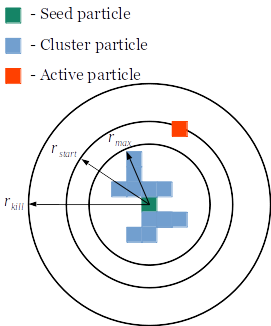
\includegraphics[width=0.95\columnwidth]{DLA_diagram.png}
  \caption{
    Diagram of the diffusion-limited aggregation (DLA) system. A particle is created at a random point on $r_{start}$ and then undergoes a discrete random walk. If its position exceeds the distance $r_{kill}$ it is removed. If it makes contact with the cluster it is made inactive and joins the cluster. The DLA cluster grows from an initial seed particle located at the origin, its size can be estimated from $r_{max}$.
  }
  \label{DLA_diagram}
\end{figure}

  Some approximations are made in this algorithm to improve computational efficiency. The original model described by Witten and Sander \cite{Witten_1981} removes particles when they reach the edge of the grid. However, this can result in significant computation spent on random walking a particle in the domain, only for it to walk to the edge and be removed. Further, if it does random walk back to a point on the circle $r_{start}$ its previous motion away from the cluster will not effect its subsequent motion. We therefore restrict the random walking to within $r_{kill}$ which still allows for some motion away from the cluster while improving overall efficiency. This restriction will have an effect on the resulting DLA cluster. However, we assume the effect is negligible for the reasons outlined.

  The random number sampling used for the random walk and the initial positions of particles generated on $r_{start}$ uses pseudo-random number generation to efficiently generate large quantities of random numbers. To ensure that the system does not generate the same cluster every time, a 'true' random number is used as the \textit{seed} of the pseudo-random number generater for each new cluster. This allows for the efficient sampling of many psuedo-random numbers that are independent between simulations, the resulting DLA clusters are consequently independent from one another.

\subsection*{Modified DLA - random adhesion}
  Previously we define \textit{checkStick()} to always be \textit{true}. However, in the modified algorithm as described by Ranguelov \textit{et al} \cite{Ranguelov_2011} we redefine \textit{checkStick()} to check against a preset probability of particle adherence $P_{stick}$, retrieving the unmodified algorithm for $P_{stick} = 1$. If the particle fails to adhere to the cluster it will do nothing until the next update where it will perform another random walk. An additional modification is made to the random walk procedure, such that if a particle tries to move into an occupied grid position it will not move and instead \textit{checkStick()} again. This prevents multiple particles from occupying a single grid space, and allows particles to have multiple 'chances' to adhere to the cluster at the same site.

\subsection*{Fractal dimension}
  A definition of dimension suitable to numerical computations of fractal dimension is the Minkowski-Bouligand or 'box-count' dimension: in a Euclidian space, the number of boxes $N$ (or 'density') with side length $a$ that cover a fractal of one dimensional size $R$ are related by
  \begin{equation}
      \begin{aligned}
        & N = (R/a)^{d_f}\\
        \implies & d_f = \frac{\ln(N)}{\ln(R/a)},
      \end{aligned}
      \label{dim_definition}
  \end{equation}

  where $d_f$ is the fractal dimension. With this definition we can retrieve well known dimensions such as $d_{line} = 1, d_{square} = 2$, etc.

      To determine the fractal dimension of the generated DLA clusters we first set $a=1$ as our DLA system is discrete in the grid, then $N=N_c$ is the number of particles in the cluster. We then assume that $r_{max}$ (the distance of the furthest point in the cluster from the origin) is representative of the one-dimensional size of the cluster with some correction terms $\alpha, \beta$. So our general relation is

  \begin{equation}
    \begin{aligned}
    & N_c(r_{max}) = (\alpha r_{max})^{d_f}+\beta\\
    \implies & \frac{d(\ln{N_c})}{d(\ln{r_{max}})} = \frac{d_f}{1 + \beta/(\alpha r_{max})^{d_f}}\\
    \implies & d_f = \lim\limits_{r_{max} \to \infty} \frac{d(\ln{N_c})}{d(\ln{r_{max}})},
    \end{aligned}
    \label{dim_relation}
  \end{equation}

  hence for sufficiently large $r_{max}$ relative to the length scale $a = 1$ we can estimate the fractal dimension $d_f$ of a DLA cluster. 

  Two methods are employed in the derivation of $d_f$ for individual DLA clusters: firstly a least squares fit method of the relationship described by (\ref{dim_relation}) is applied to the recorded values of $N_c$ and $r_{max}$ of the cluster, the corresponding $d_f$ is inferred from the fit with error; the second method approximates
  \begin{equation}
    d_f \approx \frac{\ln{N_c}}{\ln{r_{max}}}, \quad r_{max} \approx R >> a
    \label{dim_approx}
  \end{equation}
      by assuming that $r_{max}$ is sufficiently large for some $N_c$. $d_f$ is then found at the largest $N_c$ and corresponding $r_{max}$ that the cluster attains. The efficacy of these methods when applied is discussed with the results of this report.

\subsection*{Implementation}
  Please see the appendix for practical details about the specific implementation of the DLA algorithm used for this report.

\section*{Results and discussion}
  We make the assumtion that the distribution of $r_{max}$ and corresponding fractal dimension $d_f$ between many randomly sampled clusters is normal (by the central limit theorem \cite{Sadovnik_2016}) - allowing for the statistical treatment of error. Unless otherwise stated any uncertainties given will be the 95\% confidence interval on the mean. Please see the appendix for examples of clusters generated.

\subsection*{DLA cluster fractal dimension}
  Using the DLA system as described we can generate datasets from several DLA clusters of varying sizes. In particular a dataset of 100 clusters of $N_c = 20000$ particles is generated with recorded values of $N_c$ and $r_{max}$ as they grow. For this dataset and the analysis in this subsection we set $P_{stick} = 1$.

\begin{figure}[t!]
\centering
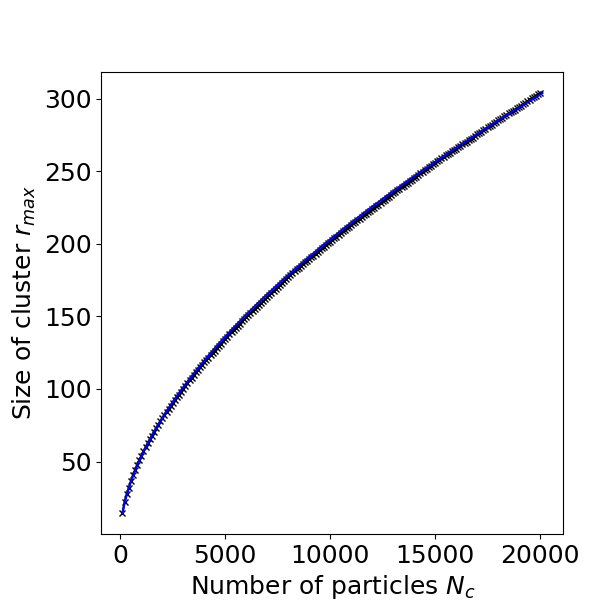
\includegraphics[width=0.95\columnwidth]{100x20k_R.png}
  \caption{
    Mean cluster size $\overbar{r_{max}}$ against particle number $N_c$ over a sample of 100 randomly generated DLA clusters. Error bars representing the 95\% confidence interval on the mean of $r_{max}$ are comparable to symbol sizes and omitted for clarity. The mean fractal dimension $\overbar{d_f}$ of the 100 cluster sample is found to be 1.733$\pm$0.004. Overlaid in blue is a plot of $N_c={\overbar{r_{max}}}^{\overbar{d_f}}$.
  }
  \label{20k_R}
\end{figure}

  Using the least squares fit method the relationship described in (\ref{dim_relation}) is fit to each DLA cluster generated and the $d_f$ are inferred. We find the mean $\overbar{d_f}$ to be 1.696$\pm$0.044, where the uncertainty includes a correction for fitting error. The mean $d_f$ from the ratio of logarithms method taken at $N_c = 20000$ on each cluster finds $\overbar{d_f} =$ 1.733 $\pm$ 0.004. The validity of the ratio of logarithms result is discussed in the following section. Both measurements agree with other literature which suggest a fractal dimension of $\sim~$1.7 in simulations \cite{Witten_1981, Choi_2011, Ranguelov_2011} and in real physical systems such as dielectric breakdown \cite{Pietronero_1984, Irurzun_2002}. A plot of the mean $r_{max} = \overbar{r_{max}}$ against $N_c$ is shown in FIG \ref{20k_R}, overlaid is a plot of $N_c={\overbar{r_{max}}}^{\overbar{d_f}}$ with the $\overbar{d_f}$ determined by the ratio of logarithms method.

  The least squares fit method has significant drawbacks that are important to consider when interpreting these results. We make the assumtion that the relationship described in (\ref{dim_relation}) holds for all scales: the dummy variables $\alpha$ and $\beta$ are included to allow for corrections, however the least squares procedure will give weight to the data at small $N_c$, which is not as representative of the fractal properties that only appear at larger cluster sizes as $r_{max} >> a=1$. There are ways of mitigating this however, e.g. for a sufficiently large cluster the fit can be applied to data that omits $N_c$ smaller than some cutoff value. Larger clusters require significantly more computation which is why we limit our dataset to just 100 generated clusters of $N_c = 20000$. This computational cost becomes a greater issue in the following section.

  A key property of fractals is their scale invariance, which our DLA model cannot reproduce for clusters of very small particle number $N_c$. This can however be useful in modelling physical systems which do have characteristic length scales and discrete particles such as electrodeposition\cite{Shaikh_2022}. Other models may also generate DLA clusters from circular particles or on non-square grids, for smaller sized clusters this can better emulate Brownian motion due to the increased degrees of freedom. However, in the limit as the cluster size increases these should all be equivalent to the Weiner process / Brownian motion.

\subsection*{Effect of random adhesion on fractal dimension}
To examine the effects of random adhesion on the fractal dimension of DLA clusters a dataset of 100 clusters per sticking probability $P_{stick}\in[0.1, 1]$ with interval 0.1 (1000 clusters total) of size $N_c = 5000$ is generated. The mean dimension is determined as in the previous section, that is $d_f$ are found for each cluster and the mean $\overbar{d_f}$ is taken over the 100 samples at each $P_{stick}$. The result is 10 values of $\overbar{d_f}$ corresponding to each $P_{stick}$. Smaller clusters than in the previous dataset are generated due to the computational cost of generating larger clusters. A smaller dataset of larger clusters was created however the statistical uncertainties in the resulting $\overbar{d_f}$ were too large ($\sim 20\%$) when using the least squares fit method.

\begin{figure}[t]
\centering
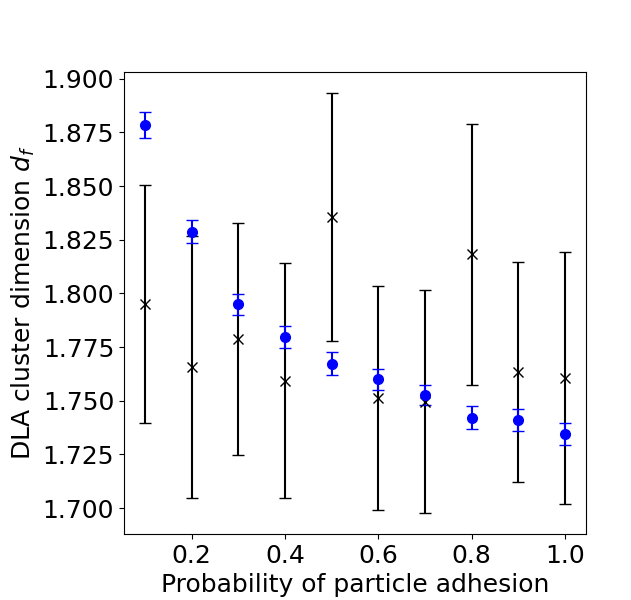
\includegraphics[width=0.95\columnwidth]{stick_dims_together.png}
  \caption{
    Derived mean fractal dimension $\overbar{d_f}$ against sticking probability $P_{stick}$. Two derivations of $\overbar{d_f}$ are shown: in blue $\overbar{d_f}$ is determined by the ratio of logarithms as in (\ref{dim_approx}) by taking the mean $d_f$ at $N_c=5000$ and corresponding $r_{max}$ of each cluster; in black $\overbar{d_f}$ is determined by fitting the relationship in (\ref{dim_relation}) to each cluster and taking the mean. In both error bars represent a 95\% confidence interval on the mean.
  }
  \label{stick_dims_together}
\end{figure}

  Both the least squares fit method and ratio of logarithms method of deriving $d_f$ are applied to this data, a comparison between the two can be seen in FIG \ref{stick_dims_together}. We can observe some striking differences in the derived $\overbar{d_f}$ between the two methods: for $P_{stick}=1$ both methods are able to reproduce within error the ratio of logarithms $\overbar{d_f}$ determined in the previous section. On this dataset at $P_{stick} = 1$ the ratio of logarithms finds $\overbar{d_f} =$ 1.735 $\pm$ 0.005 and the least squares fit finds $\overbar{d_f} = $ 1.761 $\pm$ 0.059. Note that the least squares fit method cannot reproduce its own results within error, this harms its validity.
  
  From the least squares fit method (shown in black in FIG \ref{stick_dims_together}) we see measurements of $\overbar{d_f}$ with no clear correlation, outlier values that deviate from the expected trend, and significant uncertainty. No reasonable conclusion about correlation between $d_f$ and $P_{stick}$ can be drawn from these results. On the other hand, the ratio of logarithms method shows a clear negative correlation between $d_f$ and $P_{stick}$ in line with the results of Ranguelov \textit{et al} \cite{Ranguelov_2011}. The validity of this method should not be taken for granted however, as it relies on the assumtion that measurements taken are in the limit $r_{max} >> a=1$. The small clusters in this dataset have $r_{max} \sim 10^2 \times a$, which seems to be sufficient for this approximation.

  An intuitive interpretation of this negative correlation is that: when a particle fails to adhere in a denser region of the cluster, its subsequent random motion is more likely to collide with another nearby cluster particle. This means denser 'branches' will grow faster than less dense regions in the cluster. This also allows particles to diffuse towards the centre of the cluster and fill in gaps, where they otherwise would have been 'captured' nearer to the starting radius $r_{start}$ \cite{Ranguelov_2011}. These effects overall increase the density of the generated cluster, and thus its fractal dimension.

\section*{Conclusion}

  By comparing the two methods of deriving $d_f$ over varying $P_{stick}$ and critically evaluating the results they produce, we conclude that the ratio of logarithms method is superior to the least squares fit method. The least squares fit method is unsuitable for determining $d_f$ under the conditions we have applied it because of its large statistical uncertainty and inability to reproduce its own results between similar datasets. As such, we will disregard the results from the least squares fit method in our following conclusions. In particular we will disregard its determined fractal dimension for $P_{stick} = 1$ and the lack of correlation between $\overbar{d_f}$ and $P_{stick}$ shown in FIG \ref{stick_dims_together}.

  Using the ratio of logarithms method we determin the fractal dimension of DLA clusters with sticking probability $P_{stick} = 1$ to be $\overbar{d_f} =$ 1.733 $\pm$ 0.004. Additionally we find a negative correlation between the fractal dimension $d_f$ and sticking probability $P_{stick}$ in concurrence with the literature \cite{Ranguelov_2011, Pietronero_1984}. This shows that simple changes to the DLA algorithm can have significant effects on the properties of the resulting clusters.
  
  An example application of the modified probability of adhesion algorithm to a physical system is Pietronero and Wiesmann's model for dielectric breakdown \cite{Pietronero_1984}. In the model, they give the probability of adhesion as a function of the local electric field by some relation coefficient. Their findings also show a negative correlation between fractal dimension and adhesion probability.

  Ranguelov \textit{et al} also make modifications to the radius at which the particles are generated $r_{start}(\theta)$ by setting it as a function of the radius of the cluster at angle $\theta$ + a constant. They also introduce multiple species of particles which have different probabilities of attaching to each other. The resulting clusters can vary drastically in shape and dimension. Their findings provide examples of further modifications that can be made to a DLA system to produce new fractals or better adapt the DLA algorithm to model natural phenomena.

  Further improvements could be made to our results by sampling many more clusters, and clusters of larger sizes to reduce our statistical error. This would also justify further improvements to our implementation of the algorithm that increase computational efficiency. With improving understanding of fractals and DLA systems we can hope to better model the natural processes in which they are seen.

\section*{Acknowledgements}
We would like to acknowledge the contributions of Dr A. Souslov and Dr D. Tsang for their code and resources on which the unmodified DLA model is based.

%%%References
\bibliographystyle{ieeetr}
%bibliographystyle{bathx}
\bibliography{refs}

\clearpage

\onecolumn

\section*{Appendix}

\subsection*{Example DLA clusters}

\begin{figure}[h!]
\centering
  \begin{subfigure}[t]{0.45\textwidth}
    \centering
    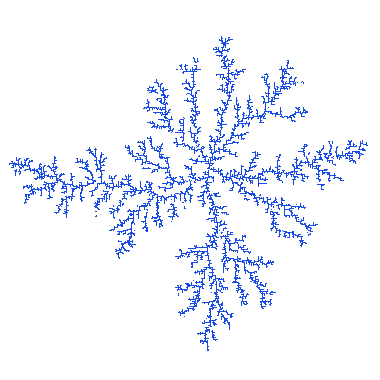
\includegraphics[width=0.95\textwidth]{p1.png}
    \caption{$P_{stick} = 1$}
  \end{subfigure}
  \hfill
  \begin{subfigure}[t]{0.45\textwidth}
    \centering
    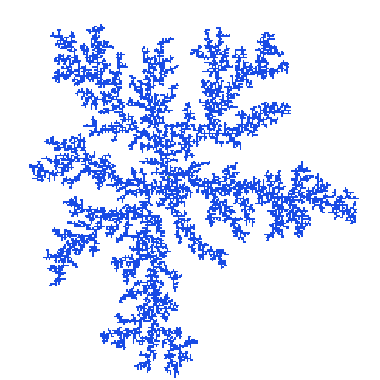
\includegraphics[width=0.95\textwidth]{p01.png}
    \caption{$P_{stick} = 0.1$}
  \end{subfigure}
  \caption{
    Example DLA clusters generated to $N_c = 10000$.
  }
\end{figure}

\subsection*{Confidence intervals}
  For the mean quantities in this report error is presented as the 95\% confidence interval on the mean given by
  \begin{equation}
    a = 1.96\frac{1}{\sqrt{n}}\sigma_x
  \end{equation}
  For some mean quantity $\overbar{x}$ where $\sigma_x$ is the standard deviation on the mean and $n$ is the number of samples. The confidence interval is then $[\overbar{x}-a, \overbar{x}+1]$. This can be interpreted as the interval such that there is a 95\% chance the interval contains the true population mean of $\overbar{x}$.

\subsection*{Implementation of algorithm}
  The DLA data discussed in this report was generated by an implementation of the described DLA algorithm in C++. Standard C++ libraries are used for sampling of 'true' and psuedo-random numbers used in the random walk and particle generation. Utilities were written to record multiple simulations with varying parameters and to export recorded data from simulations to a csv format. Data analysis and derivation of fractal dimension was performed in Python using the numpy and pandas libraries. All computations were performed on a 64-bit desktop processor running Linux Mint 20.1 'Ulyssa'.

  \textbf{Note: when compiling and running the C++ code provided, the makefile in 'source' has been edited. To compile the code place the .cpp and .h files into a directory called 'source' and add in the missing/unedited files (Particle.h, Window.h, Window.cpp). Run 'make -B -C ./source/' from the directory above 'source'. The compiled binary and the data it produces are in this directory, execute the binary using './run'. The python data analysis file 'DLA.py' should also be run from this same directory}

  The changes made to the C++ code given by Dr A. Souslov and Dr D. Tsang are spread throughout the source code provided (i.e: CSVWrite.h, DLASystem.cpp, DLASystem.h, mainDLA.cpp, rnd.h, Makefile). Most of the changes made are used when pressing 't' in the simulation window to set parameters for data recording and $P_{stick}$ etc. Some new functions have been added to the DLASystem class, and a new class CSVWrite is written for data recording. Some select functions are presented here but you would do best to look at the source code with comments.

\begin{lstlisting}
// check if the last particle should stick (to a neighbour)
int DLASystem::checkStick() {
	Particle *lastP = particleList[numParticles - 1];
	int result = 0;
	// loop over neighbours
	for (int i = 0; i < 4; i++) {
		double checkpos[2];
		setPosNeighbour(checkpos, lastP->pos, i);
		// if the neighbour is occupied...
		if (readGrid(checkpos) == 1)
      if(randomStick){
	      double rr = static_cast<double>(rgen.randomInt(1000));
        if (static_cast<double>(rr/1000.0) < stickChance){result = 1;}
        else {result = 0;}
      }
      else {result = 1;}
	}
	return result;
}
\end{lstlisting}

\begin{lstlisting}
void DLASystem::recordData(int numOfSims, int nInterval_, pair<int, int> nRange_) {
  if(running != 0 && !recording){cout << "please pause simulation before recording data" << endl;}
  else{ 
    if (numOfSims >= 2){
      cout << "Starting DLA multiple recording" << endl;
      simNum = numOfSims;
      numSims = numOfSims;
    }else cout << "Starting DLA recording" << endl;
    
    recording = true;

    nInterval = nInterval_;
    nRange = nRange_;
  }
}
\end{lstlisting}

\begin{lstlisting}
//record data on update
void DLASystem::updateRecording() {
  if(numParticles == nRange.second){
    //cout << "recording data at N = " << numParticles << endl;
    numData->push_back(static_cast<double>(numParticles));
    radiusData->push_back(clusterRadius);

    if (simNum == numSims) {dataSet->push_back(*numData);} //only need one column of this

    //when finished in range write data to dataSet \& reset sim
    if (simNum >= 1){
      dataSet->push_back(*radiusData);
      cout << "Sucessfully recorded sim number " << simNum << " data in range (" << nRange.first << ", " << nRange.second << ") with interval " << nInterval << endl;

      //reset initial conditions
      Reset(); //will reset numData and radiusData
      setRandomSeed();
      setFast();

      if (simStickNum != 0 && simNum \% simStickNum == 1 && simNum != numSims){
        if (stickDiff != 0){
          stickChance -= stickDiff;
          if(stickChance<=0){
            cout << "sticking chance is now 0, finishing recording" << endl;
            writeDataCSV();
            recording = false;
            pauseRunning();
          }
          else cout << "new sticking chance set to " << stickChance << endl;
        }
      }

      setRunning();

      if (simNum == 1) {writeDataCSV();}

      simNum--;
      //cout << "conditions reset for simulation number " << simNum << endl;
    }

    if (simNum <= 0) {recording = false; pauseRunning();}
  }
  else if(numParticles > nRange.first
          && numParticles % nInterval == 0
          && numParticles > numData->size() * nInterval + nRange.first){
    //cout << "recording data at N = " << numParticles << endl;
    numData->push_back(static_cast<double>(numParticles)); //dont really need to do this...
    radiusData->push_back(clusterRadius);
  }
}
\end{lstlisting}

\begin{lstlisting}
//write recorded data to a CSV file
void DLASystem::writeDataCSV(){
  auto csv = new CSVWrite("./data.csv");

  csv->WriteVector(dataSet);
  csv->CSVClose();

  //clearDataSet();

  recording = false; //should be false anyways
}
\end{lstlisting}

\end{document}
